\documentclass[a4paper]{article}
\usepackage[newfloat]{minted}
\usepackage{graphicx}
\usepackage{caption}
\usepackage[a4paper,left=3cm,right=2cm,top=2.5cm,bottom=2.5cm]{geometry}
\usepackage[colorlinks=true, urlcolor=blue, pdfborder={0 0 0}]{hyperref}
\newenvironment{code}{\captionsetup{type=listing}}{}
\SetupFloatingEnvironment{listing}{name=Code}

\title{RL Homework 1}
\author{Ananth Mahadevan}
\begin{document}
\maketitle
\clearpage
\tableofcontents
\clearpage

\section{Question 1}
\textbf{Question}:\\
Can the same model, trained with 200 timesteps, balance the pole for 500 timesteps? Why/why not?
\\
\textbf{Answer}:\\
Yes if the model that is trained for 200 timesteps is able to generalize well enough to balance the pole, then the model will also be able to balance the pole for 500 timesteps. This can be verified easily by running the test with the \textit{CartPole-v0\_params\_basic} model parameters

\section{Queston 2}
\textbf{Question:}\\
Why is there a very large variance in 100 independent training runs?What is the implication of this, when it comes to comparing reinforcement learning algorithms to each other?
\\
\textbf{Answer:}\\
The reason that the 100 runs have a high variance is due to the stochastic nature of the training environment. As every restart makes the pole start in slightly different scenario, the policy that might have been learnt will differ largely. In one training run, the optimal policy might be learnt in the first 100 episodes while in another run it might not converge to an optimal policy at all. This results in large variance between runs.

This is a big issue as then we need to compare RL algorithms on an average ability to train an agent and not on individual training runs as the variance is large it might lead to incorrect results. This means that it becomes computationally harder to compare different RL algorithms.

\section{Question 3}
\subsection{Incentive to stay at centre $x=0$}
    The reward function that was created was one that gives most for staying at $x=0$ and decreases reward as it moves away from 0. The function is seen in Code~\ref{code:reward-0}
    \begin{code}
        \captionof{listing}{Reward function for $x=0$}
        \label{code:reward-0}
    \begin{minted}{python}
        def new_reward(state):
            return 1/(1+(state[0])**2) 
    \end{minted}
    \end{code}
    This results in a reward function as seen in Figure~\ref{fig:reward-0}
    \begin{figure}[ht!]
        \centering
        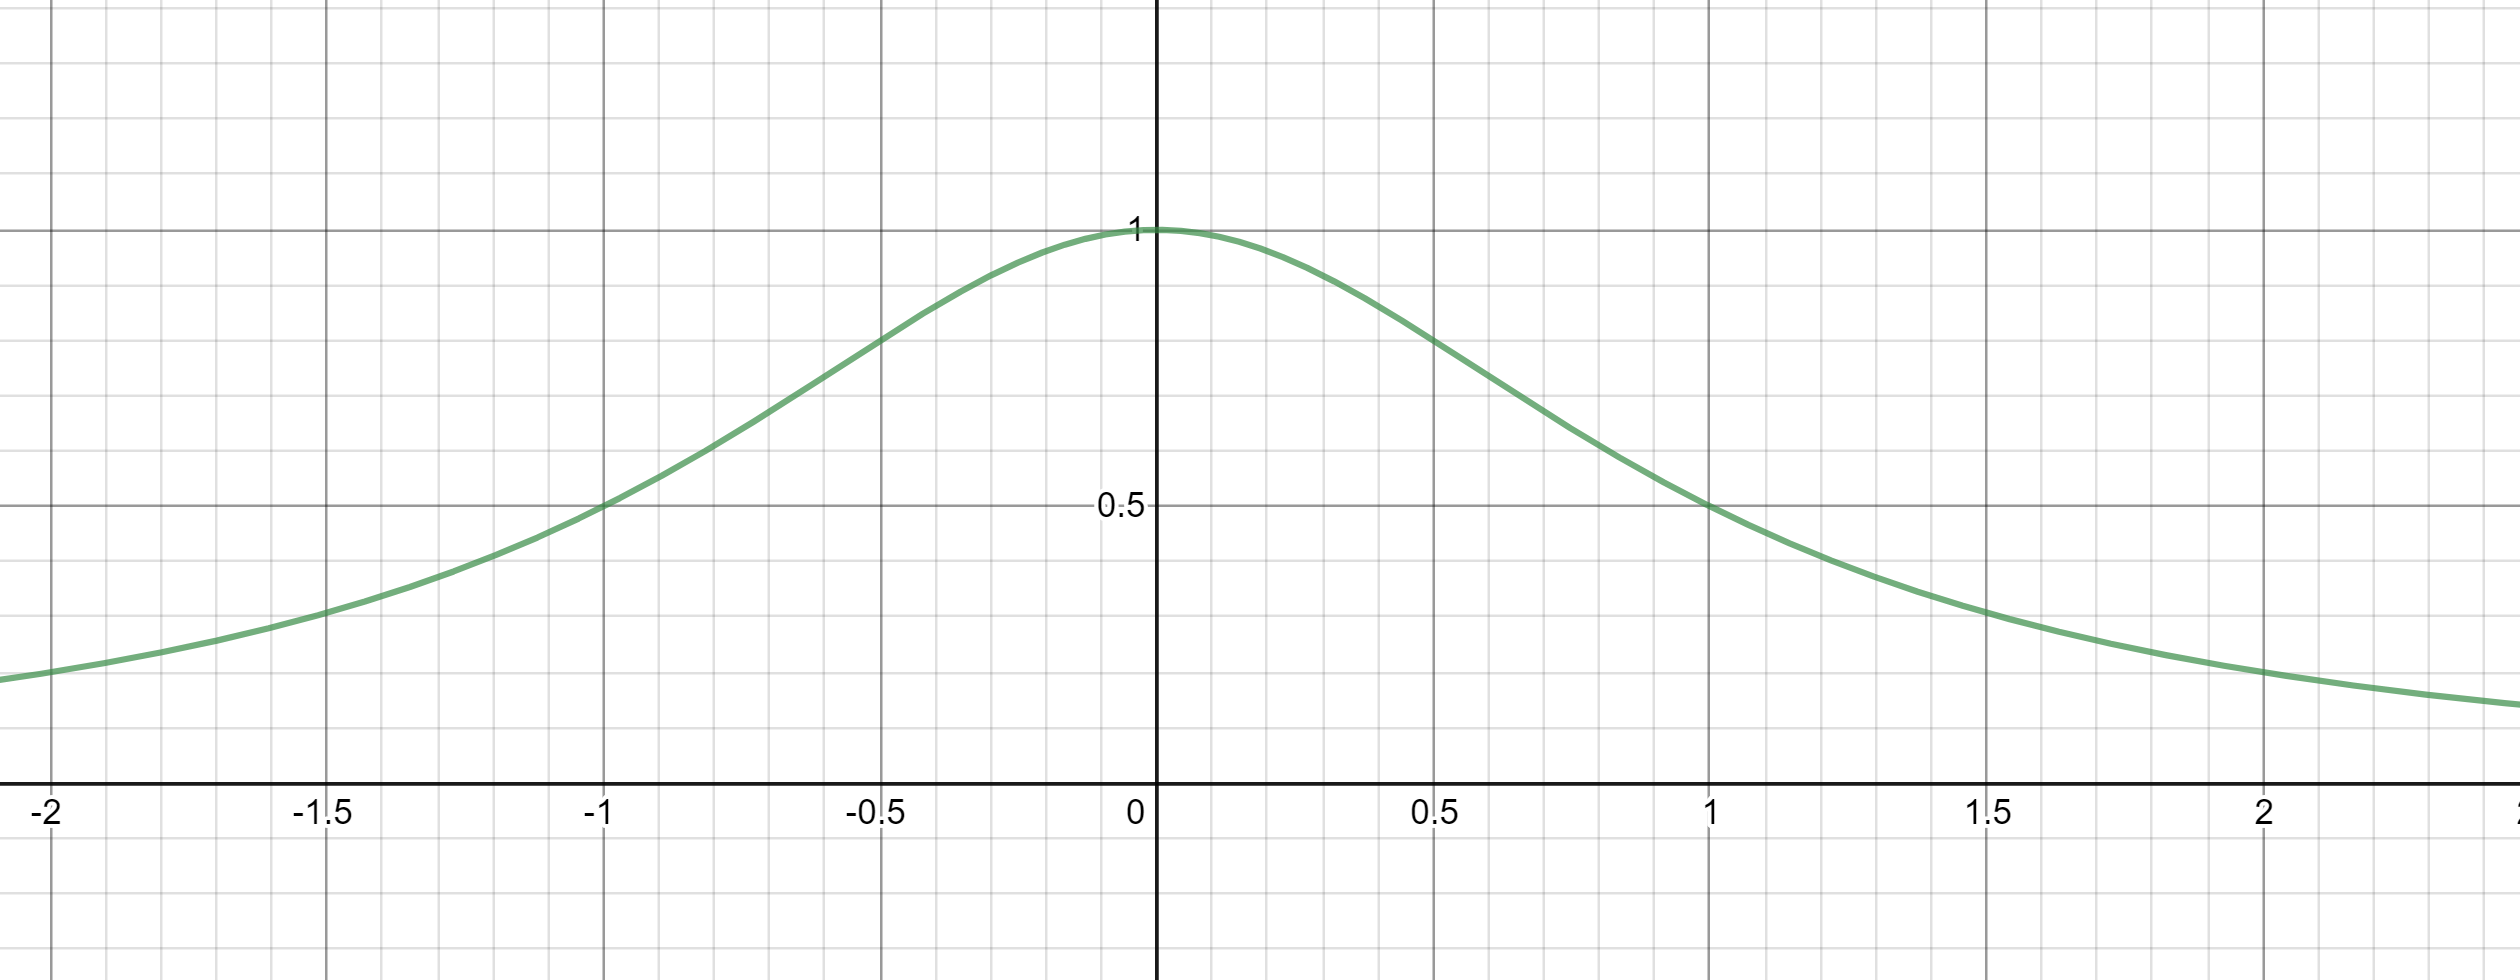
\includegraphics[width=\textwidth]{center.PNG}
        \caption{Reward function for $x0=0$. Here x-axis is position of agent}
        \label{fig:reward-0}
    \end{figure}
    This can be verified using the \textit{CartPole-v0\_params\_x0\_0} model.
\subsection{Incentive to stay at $x=x_0$}
    This task was somewhat more complex as there needs to be enough incentive for the pole to remain upright along with incentive to move towards the location. Then rewards must also be reduced so that the agent "sticks" to the location once it reaches it.
    Initially a reward function worked for training at staying at $x=2$, but then the logic didn't generalize when training for any $x_0$. The function was something as seen in Figure~\ref{fig:kinda}
    \begin{figure}[ht!]
        \centering
        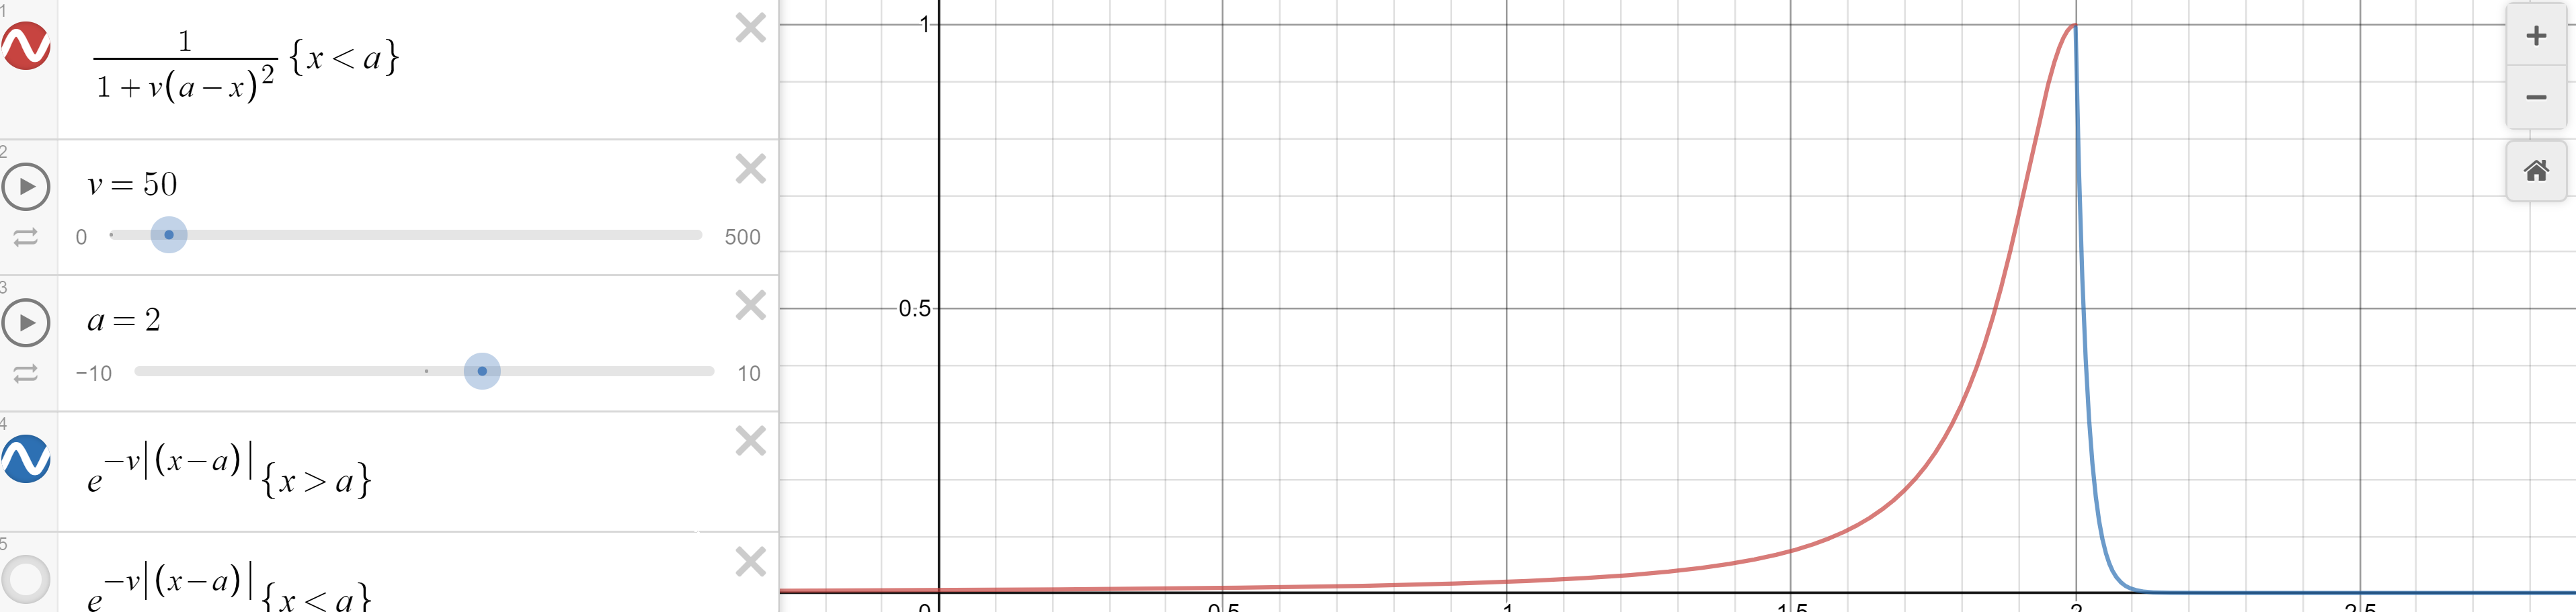
\includegraphics[width=\textwidth]{other_reward.PNG}
        \caption{Complex piecewise reward function for $x=2$ which kinda worked. Here x-axis is position of agent }
        \label{fig:kinda}
    \end{figure}  


    But the general reward function was not feasible for any $x=x_0$ as seen in the function Code~\ref{code:fail}
    \begin{code}
        \captionof{listing}{Failed reward function for $x=x_0$}
        \label{code:fail}
        \begin{minted}{python}
            def x0_reward(state,x0):
            if x0 >= 0:
            if state[0]<=x0:
            return 1/(1+20*(x0-state[0])**2)
            else:
            return np.power(np.e,-100*np.abs(state[0]-x0))
            else:
            if state[0]<=x0:
            return np.power(np.e,-100*np.abs(state[0]-x0))
            else:
            return 1/(1+20*(x0-state[0])**2)
        \end{minted}
    \end{code}
    These kind of incentives did not seem to converge to any optimal agent and was having high variance. Then I returned to use a simple reward function similar to Code~\ref{fig:reward-0} but centered around a specific value of $x_{0}$, the challenge was decreasing the variance of the function to make sure the agent stays fixed at a location. The reward function is as seen in Code~\ref{code:x0}
    \begin{code}
        \captionof{listing}{Reward function for $x=x_0$}
        \label{code:x0}
        \begin{minted}{python}
            def new_reward(state,x0):
                return 1/(1+200*(x0-state[0])**2)
        \end{minted}
    \end{code}
    The $200$ is to make the variance of te reward function small enough as seen in Figure~\ref{fig:x0-1} which is much sharper than Figure~\ref{fig:reward-0}
    \begin{figure}[ht!]
        \centering
        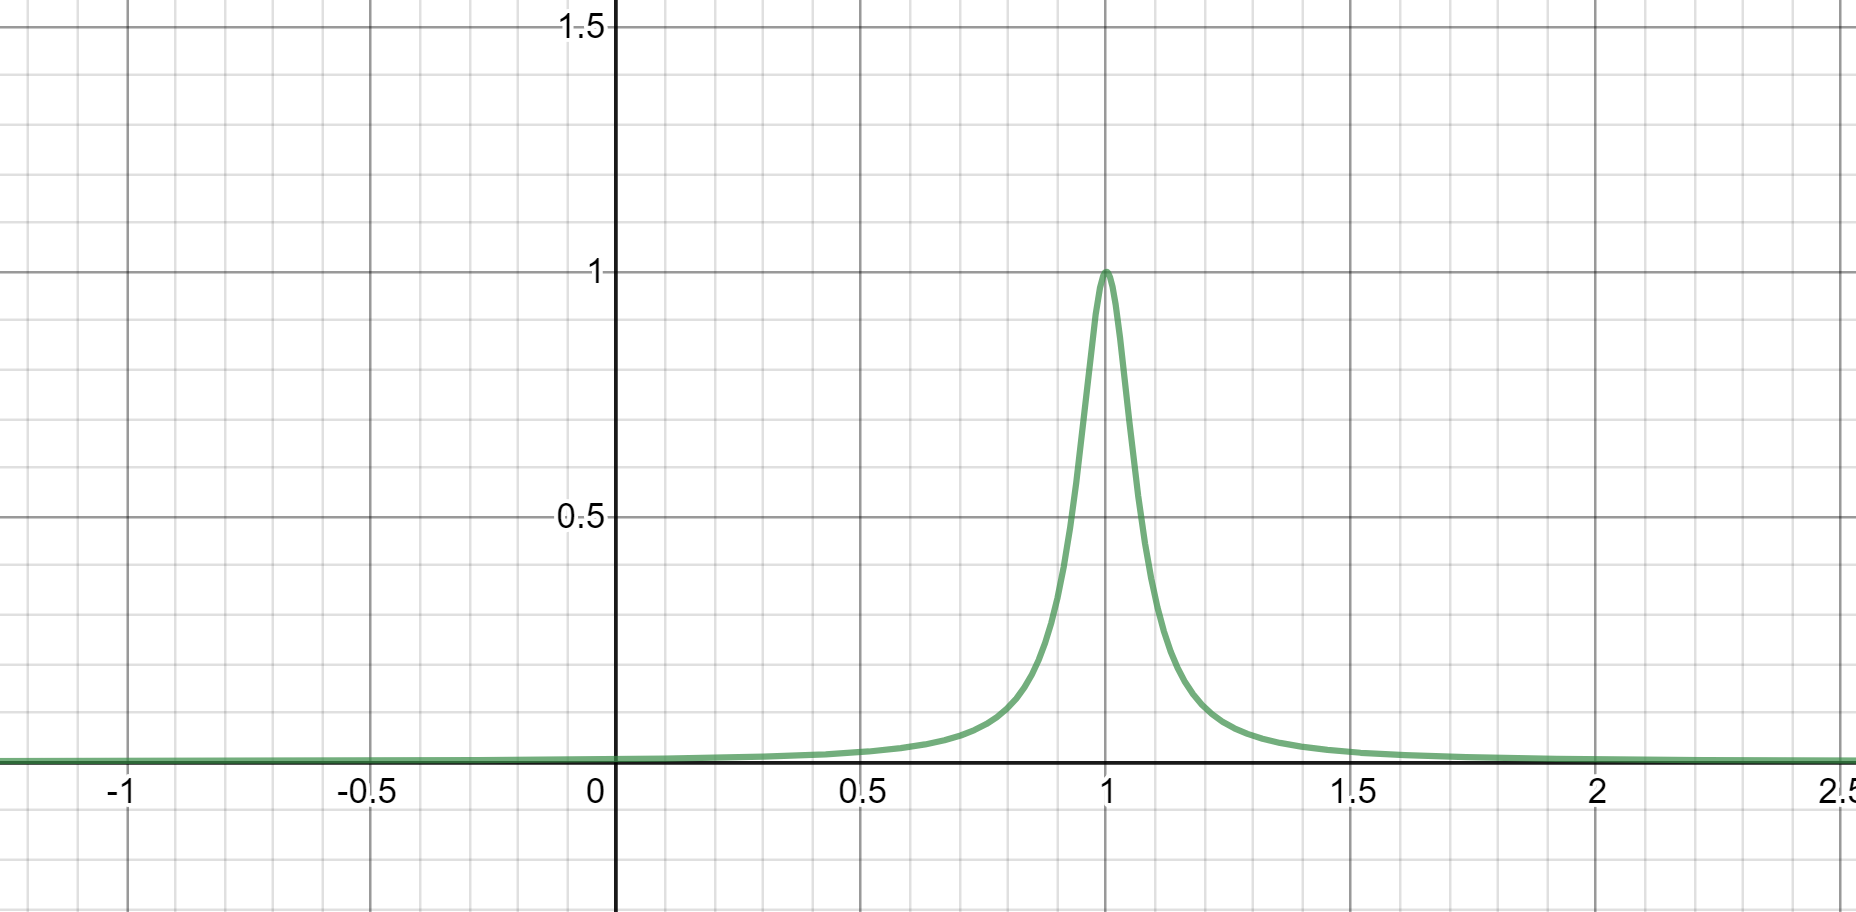
\includegraphics[width=\textwidth]{x0.PNG}
        \caption{Reward function for $x0=1$ (specifically). Here x-axis is position of agent}
        \label{fig:x0-1}
    \end{figure}
    The model trained for $x_0=1$ and can be verified using the \textit{CartPole-v0\_params\_x0\_1} model parameters.
\subsection{Incentive to keep moving cart as fast as possible}
This task too was interesting for the fact that going fast and staying alive are slightly orthogonal for the agent. This means there must be sufficient reward for staying alive in each timestep and at the same time moving fast. Learning from previous approaches I designed a simple function which uses the property of $tanh(x)$ function which effectively caps the speed and then taking the absolute so that speed in either direction was rewarded equally. Then finally the value was scaled so that the reward function uses a  $30:70$ ratio of giving priority to speed. The reward function is seen in Code~\ref{code:speed}
\begin{code}[ht]
    \captionof{listing}{Reward function for speed}
    \label{code:speed}
    \begin{minted}{python}
        def fast_reward(state):
            return  0.3 + 0.7*np.abs(np.tanh(state[1]/2)) 
    \end{minted}
\end{code}
The reward function is as seen in Figure~
\begin{figure}[ht!]
    \centering
    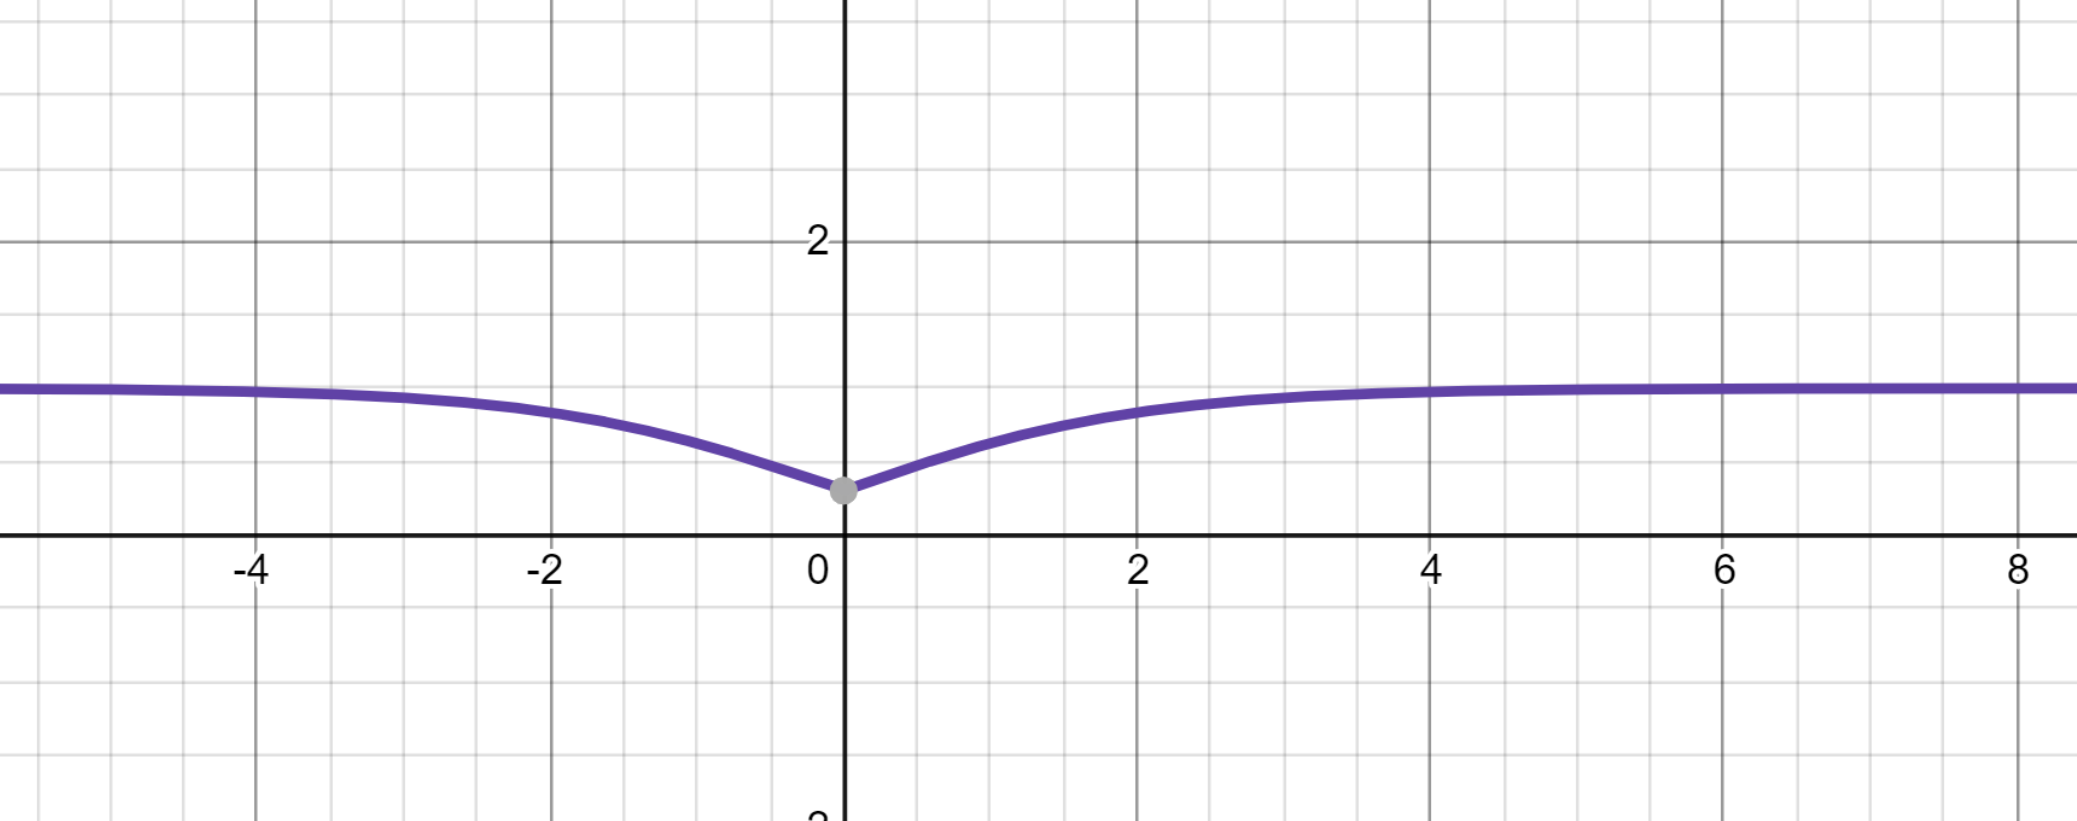
\includegraphics[width=\textwidth]{speed.PNG}
    \caption{Reward function for speed. Here x-axis is speed of agent}
    \label{fig:speed}
\end{figure}
The results are nice, the agent learns to oscillate between left and right and achieves a decent speed. There might be a better reward function that allows the agent to learn a faster movement. The agent is found in file \textit{CartPole-v0\_params\_faster\_better.mdl}.

\subsection{Answer}
\textbf{Question:}\\
How does canging the reward function impact the time for training?
\\
\textbf{Answer:}\\
Once the reward function was changed the agent needed to learn a more complex policy which would allow it to achieve the tasks set out. This usually meant that the agent must be trained for longer number of timesteps so that a trivial solution is not reached along with training for a larger number of episodes as the agents took much more time to converge to a solution.

The reason is mostly because the reward function gets more complex and the agent must explore more to find optimal policy. This takes more time the more complex the task is. 

\end{document}